\documentclass{tudelft-report}

%% Set up the bibliography
\usepackage{biblatex}
\usepackage[utf8]{inputenc}
\usepackage{enumitem} 
\usepackage{titlesec} % For title formatting
\usepackage{comment}
\usepackage{tabularx}
\addbibresource{report.bib}

%% Additional packages and commands
\usepackage{parskip}
\setlist{itemsep=-2pt} % Reducing white space in lists slightly
\renewcommand{\deg}{\si{\degree}\xspace} % Use \deg easily, everywhere

\usepackage{hyperref}
\hypersetup{
    colorlinks=true,
    linkcolor=blue,
    filecolor=magenta,      
    urlcolor=cyan,
    pdftitle={Overleaf Example},
    pdfpagemode=FullScreen,
    }

\urlstyle{same}

% Define the instruction box style
\specialcomment{instruction}{\begingroup\color{red}\itshape}{\endgroup}
\excludecomment{instruction} % Exclude all instructions from printing

%% ----------------------------------------------------------------------
%%    Begin of document + Frontmatter (Roman page numbering)
%% ----------------------------------------------------------------------

\begin{document}

\frontmatter

%% Define the main parameters
\title{IOF Core Patterns}
\subtitle{A compendium of Semantic Data Patterns based on IOF Core}
\author{Author1 \\ Author2}

\subject{Draft} % Cover only
\affiliation{NIST} % Cover only
\coverimage{figures/College-Cover-Page.pdf} % Aspect ratio of 2:3 (portrait) recommended
\definecolor{title}{HTML}{fee7dd} % Color for cover title

\makecover

\begin{titlepage}

\begin{center}

%% Print the title
{\makeatletter
\largetitlestyle\fontsize{45}{45}\selectfont\@title
\makeatother}

%% Print the subtitle
{\makeatletter
\ifdefvoid{\@subtitle}{}{\bigskip\titlestyle\fontsize{20}{20}\selectfont\@subtitle}
\makeatother}

\bigskip
\bigskip

by

\bigskip
\bigskip

%% Print the name of the author
{\makeatletter
\largetitlestyle\fontsize{25}{25}\selectfont\@author
\makeatother}

\bigskip
\bigskip

%% Print table with names; easily add columns if necessary or remove the table completely
\setlength\extrarowheight{2pt}
% \begin{tabular}{l}
    % Editor: TBD \\\midrule
    % Contributors: TBD  \\
% \end{tabular}

\vfill

%% Print some more information at the bottom
\begin{tabular}{ll}
    Authors: & I. Surname \\
    Editors: & I. Surname \\
    Proofread by: &  I. Surname1, I. Surname2
\end{tabular}

\bigskip
\bigskip

%% Add a source and description for the cover and optional attribution for the template
\begin{tabular}{p{15mm}p{10cm}}
    Copyright: & (c) 2025, Open Applications Group   \\
    % Feel free to remove the following attribution, it is not required - still appreciated :-)
    Release:  & 2025
\end{tabular}

\end{center}

%% Insert the TU Delft logo at the bottom of the page
\begin{tikzpicture}[remember picture, overlay]
    \node[above=10mm] at (current page.south) {%
        
\includegraphics[scale=0.3]{figures/OAGi-IOF.png}
    };
\end{tikzpicture}

\end{titlepage}

\chapter*{Preface}
\addcontentsline{toc}{chapter}{Preface}

\emph{A preface...}

\begin{flushright}
{\makeatletter\itshape
    \@author \\
    \monthname{} \the\year{}
\makeatother}
\end{flushright}

\chapter*{Summary}
\addcontentsline{toc}{chapter}{Summary}

summary of the compendium ...










\tableofcontents
%\listoffigures
%\listoftables

\chapter*{Glossary}
\addcontentsline{toc}{chapter}{Glossary}

\emph{List all domain-specific, technical, other abbreviations and internally standardised terms in the glossary, e.g., construct - we mean terms in IOF. \\ 
DO NOT include ontology constructs including BFO or IOF in the glossary.}

\noindent
\setlist[description]{style=nextline, labelwidth=0pt, leftmargin=1.5em, labelsep=0.9em} % Customize hanging indent
\begin{description}
    \item[\textbf{aliquam}] 
    \hspace{3mm} tincidunt urna. Nulla ullamcorper vestibulum turpis. Pellentesque cursus luctus mauris.
    
    \item[\textbf{cras viverra}]
    \hspace{3em} metus rhoncus sem. Nulla et lectus vestibulum urna fringilla ultrices. Phasellus eu tellus sit amet tortor gravida placerat.
    
    \item[\textbf{donec nonummy}]
    \hspace{3em} pellentesque ante. Phasellus adipiscing semper elit. Proin fermentum massa ac quam. Sed diam turpis, molestie vitae, placerat a, molestie nec, leo.
    
    \item[\textbf{integer sapien}]
    \hspace{3em} est, iaculis in, pretium quis, viverra ac, nunc. Praesent eget sem vel leo ultrices bibendum. Aenean faucibus.
    
    \item[\textbf{lorem ipsum}]
    \hspace{3em} dolor sit amet, consectetur adipiscing elit. Ut purus elit, vestibulum ut, placerat ac, adipiscing vitae, felis. Curabitur dictum gravida mauris.
\end{description}




%% ----------------------------------------------------------------------
%%    Mainmatter (Arabic page numbering)
%% ----------------------------------------------------------------------

\mainmatter

\chapter{Introduction}
\label{chapter:introduction}
% Instruction box
\textit{
This chapter is for everything we need to inform in general before presenting the patterns.
}


\section*{Purpose and scope}
\addcontentsline{toc}{section}{Purpose and scope}

\section*{Basic Formal Ontology (BFO)}
\addcontentsline{toc}{section}{Basic Formal Ontology}

\section*{IOF Core}
\addcontentsline{toc}{section}{IOF Core}


\section*{How to use the patterns}
\addcontentsline{toc}{section}{How to use the patterns}

\subsection*{Identify the correct patterns to use}
\addcontentsline{toc}{section}{Identify the correct patterns to use}


\subsection*{Use in Data mapping}
How to use the INSERT DATA mapping (adopt and adjust) 

\subsection*{Use in Data validation}
SPARQL and SHACL

\subsection*{Extension and customization}
understand the general pattern
Explore how different patterns can be combined.

\section*{Versioning and changes}


%\input{mainmatter/chapter-4} % Create file to add

%% ----------------------------------------------------------------------
%%    Aspects and scenerios
%% ----------------------------------------------------------------------
\textit{
Only add aspects that are main chapters. Each scenario will be a section with TOC entry only with the scenario name. Compile scenarios under the aspect chapters below.
}



\chapter{Time}

\section{Associate clock time and calendar date}
\section{Clock time and calendar date}
\label{sec-clock-calendar}

\textbf{Created by:} Arkopaul Sarkar \\
\textbf{Modified by:} Arkopaul Sarkar \\

\subsection*{Scenario Objective}

This scenario illustrates how to associate clock time and calendar dates with instances of time. While the ability to store clock time and calendar dates allows users to perform various quantitative analyses on the processes and their durations, the wide variety of clock and calendar systems presents challenges in accurately representing dates and times in the correct format. We include use cases depicting both basic and advanced methods for representing date and time values of temporal instances.


\subsection*{General Pattern Description}

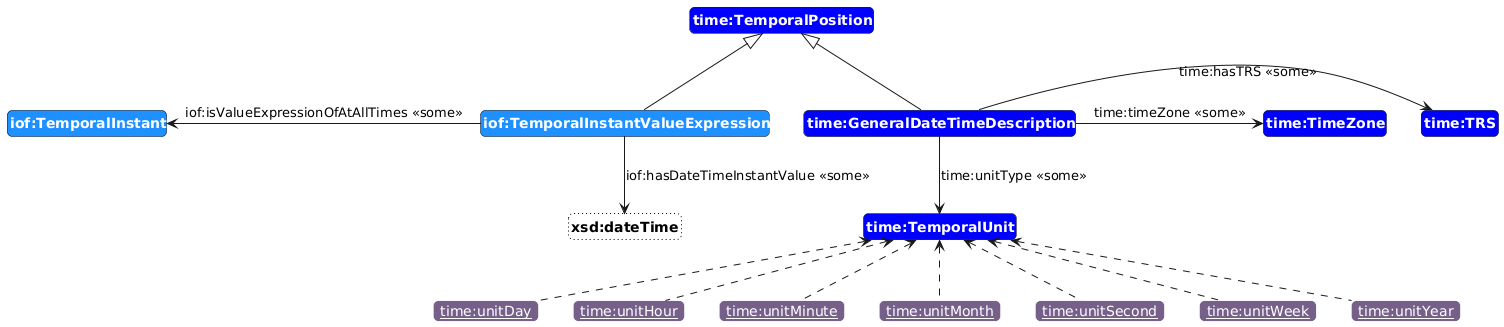
\includegraphics[scale=0.28]{scenarios/clock-time-calendar-date/images/general-clock-calendar.png}

the calendar and clock time for a specific temporal instant can be expressed by associating different instances of the information class \texttt{iof-core:TemporalInstantValueExpression} or OWL-Time class \texttt{time:General\\DateTimeDescription} as both are subclass of \texttt{time:TemporalPosition} (\texttt{iof-core:TemporalInstantValue\\Expression} is mapped as subclass of \texttt{time:TemporalPosition}.  

\subsubsection*{Use Case: Launch of first iPhone} 
The original iPhone was first released on June 29, 2007. 

The date and time of the launch are captured in 1) XSD dateTime format, 2) in a specific time zone, and 3) using a custom date and time format. The process \texttt{launch-of-iphone} is not detailed further except the temporal interval it occupies. This instance of temporal interval is then connected to its first temporal instant, for which the calendar date and clock time are assigned.   

\subsubsection*{Use-Case Pattern Description}

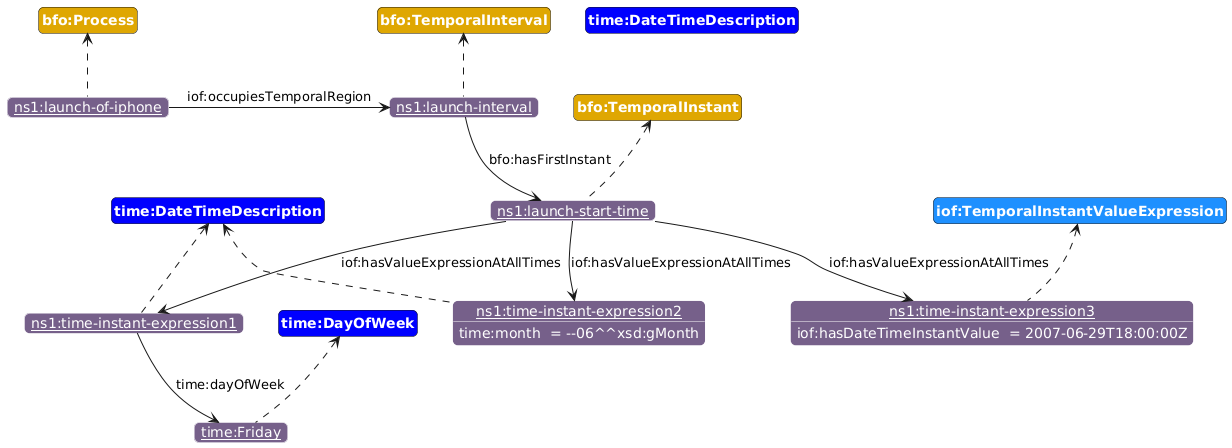
\includegraphics[scale=0.35]{scenarios/clock-time-calendar-date/images/uc1-dow-mn.png}

The launch date and time are expressed in three different ways.  

\texttt{hasDateTimeInstantValue} can associate the date and time value in \texttt{xsd:dateTime} format. If the date and time values can be expressed in XSD format, this pattern does not require any reference to OWL Time ontology. Also, \texttt{xsd:dateTime} format already has provision for mentioning time zone (e.g., 2007-06-29T14:00:00-04:00 which has a UTC-4 time zone offset for EDT). However, as XSD:dateTime datatype is the range of \texttt{iof-core:hasDateTimeInstantValue}, no other XSD type or a different format can be expressed using this pattern. 

\paragraph{Other components of a clock time \\}

In the above pattern, the launch date and time of the iPhone in New York are expressed as `day of the week' using \texttt{time:dayOfWeek} (OWL Time ontology provides the days of a week as instances of type \texttt{time:DayOfWeek})  and `month', using \texttt{time:month} data property \texttt{xsd:gMonth} which links to an indexical value based on the order of months in the calendar of type \texttt{xsd:gMonth} \footnote{\url{https://www.w3.org/TR/xmlschema11-2/\#gMonth}}.
Various combinations of data properties of \texttt{time:GeneralDateTimeDescription}, e.g.,  year, month, day, hour, minute, and second, can be used to express a clock time or calendar date, e.g., only date value in year, month and day. The corresponding time zone can be mentioned by linking an instance of \texttt{TimeZone} \footnote{For detailed guidance about working with time zones, see \url{http://www.w3.org/TR/timezone/} .}, using \texttt{time:timeZone} property.       

\paragraph{Using custom clock time format \\}

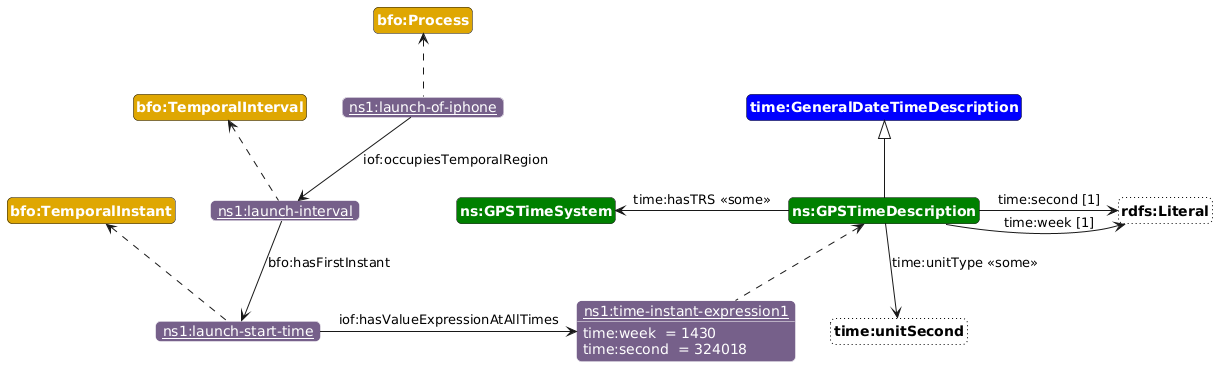
\includegraphics[scale=0.35]{scenarios/clock-time-calendar-date/images/uc1-custom.png}

In the above pattern the launch date is expressed in `GPS time'. As GPS time is the number of seconds since an epoch in 1980, encoded as the number of weeks and seconds into the week, the new class  \texttt{GPSTimeDescription}, extended from \texttt{time:DateTimeDescription}, should contain values for data properties \texttt{time:second} and \texttt{time:week}. The example does not provide details of \texttt{GPSTimeSystem}, which is a \texttt{time:TemporalReferenceSystem}, and may refer to a suitable description of `GPS time', e.g., A taxonomy of temporal reference systems is provided in ISO 19108:2002. 


\subsubsection*{Data Mapping Description}

\begin{verbatim}
INSERT DATA {
    ns1:launch-of-iphone a bfo:Process;
                        bfo:occupiesTemporalRegion ns1:launch-interval.
    ns1:launch-interval a bfo:TemporalInterval;
                        iof:hasFirstInstant ns1:launch-start-time.
    ns1:launch-start-time a bfo:TemporalInstant;
                        iof:hasValueExpressionAtAllTimes ns1:instant-expression-xsd;
                        iof:hasValueExpressionAtAllTimes ns1:instant-expression-month;
                        iof:hasValueExpressionAtAllTimes ns1:instant-expression-dow;
                        iof:hasValueExpressionAtAllTimes ns1:instant-expression-gps.
    ns1:instant-expression-xsd a iof:TemporalInstantValueExpression;
                        iof:hasDateTimeInstantValue "2007-06-29T18:00:00Z"^^xsd:dateTime.
    ns1:instant-expression-month a time:DateTimeDescription;
                        time:month "--06"^^xsd:gMonth.
    ns1:instant-expression-dow a time:DateTimeDescription;
                        time:dayOfWeek time:Friday.
    ns1:instant-expression-gps a ns:GPSTimeDescription;
                        time:week "1430"^^xsd:decimal;
                        time:second "324018"^^xsd:decimal. 
}
\end{verbatim}

\texttt{ns:GPSTimeDescription} class has a temporal reference system as \texttt{ns:GPSTimeSystem}, which refer to the specification of GPS time format. Following the standard, a \texttt{GPSTimeDescription} has a 

e\begin{verbatim}
:GPSTimeDescription rdf:type owl:Class ;
    rdfs:subClassOf 
    <http://www.w3.org/2006/time#GeneralDateTimeDescription> ,
    [ rdf:type owl:Restriction ;
        owl:onProperty <http://www.w3.org/2006/time#hasTRS> ;
        owl:hasValue :GPSTimeSystem
    ] ,
    [ rdf:type owl:Restriction ;
        owl:onProperty <http://www.w3.org/2006/time#unitType> ;
        owl:hasValue <http://www.w3.org/2006/time#unitSecond>
    ] .    

:GPSTimeSystem rdf:type owl:NamedIndividual ,
    <http://www.w3.org/2006/time#TRS> ;
    AnnotationVocabulary:adaptedFrom "https://en.wikipedia.org/?title=GPS_time" .
\end{verbatim}


\subsubsection*{Data Validation}



\section{How to integrate different clock and calendar systems}
\chapter{Objects, artifacts and their materials}

\section{What an Object is Made of}
\label{chapter-scenario-template}
\textit{This template should be used to create a scenario. Please copy to a dedicated folder under folder `scenario'. All images should be referred from `image' folder under the dedicated folder. For example, please see: \\
\cref{sec-change-location}}

\section*{<Scenario title>}


\textbf{Created by:} Perawit Charoenwut \\
\textbf{Modified by:} Perawit Charoenwut \\

\subsection*{Scenario Objective}


\subsection*{General Pattern Description}





\subsection*{Use Case: <Use-Case title>}

\subsubsection*{Use-Case Pattern Description}

\subsubsection*{Use-Case Example Data}


\subsubsection*{Data Mapping}


\subsubsection*{Data Validation}



\chapter{assembly-component}

\section{components of an assembly}

A car engine is often showcased in parts: pistons, crankshaft, cylinders

An insulated wall comprises drywall, insulation foam, and outer sheathing.

Sewing patches of silk, cotton and leather make an item of clothing.

\section{Embedded components}

Reinforcement Bars in Concrete Structures

coating on a metal surface

printed circuit on board

Embedded sensors

\section{being components of different assemblies at different times}

A bulb can be a component of different lighting fixtures.

\section{being components of different assemblies at the same times}

door is a component of both room.

\section{Temporary components}

Each stage of the rocket is only part of the whole vehicle for a specific phase of the journey

\section {Components as an identity of the assembly}

Changing the battery of a wall clock or the tire of a car does not change the wall clock or the car.

But changing the CPU changes the laptop. 









\chapter{Person and agent}

\section{Different types of agents}
\label{chapter-scenario-template}
\textbf{Created by:} Perawit Charoenwut \\
\textbf{Modified by:}

\subsection*{Scenario Objective}
This scenario aims to demonstrate how to model relationships between different types of agents in commercial transactions using the IOF Core patterns. The pattern models how different entities (such as persons and organizations) can take on specific roles (such as buyer and supplier) within complementary business processes that involve material products. This pattern is fundamental for representing any transaction where one party acquires a product from another, making it clear which agents are involved and what their specific roles are within the transaction context.

\subsection*{General Pattern Description}
The pattern models the relationship between buyers, suppliers, and material products through their roles and participation in business processes. It demonstrates how:

An agent classified as a Buyer has a BuyerRole that participates in a BuyingBusinessProcess
An agent classified as a Supplier has a SupplierRole that participates in a SupplyingBusinessProcess
Both business processes have the same MaterialProduct as a participant

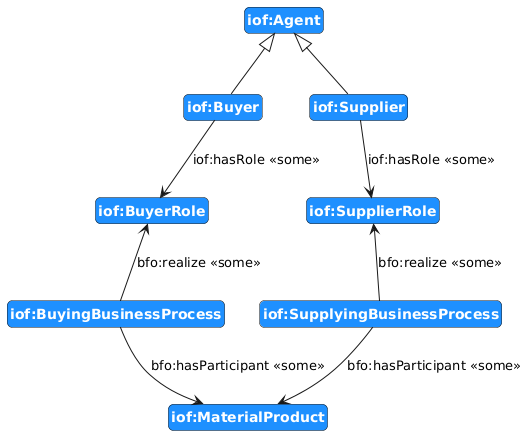
\includegraphics[scale=0.4]{scenarios/different-type-agent/image/different-type-agent-schema.png}

\subsection*{Use Case: Coffee Shop Transaction}
\subsubsection*{Use-Case Pattern Description}
This use case demonstrates how a buyer (John), purchases a cup of coffee from a cafe. 

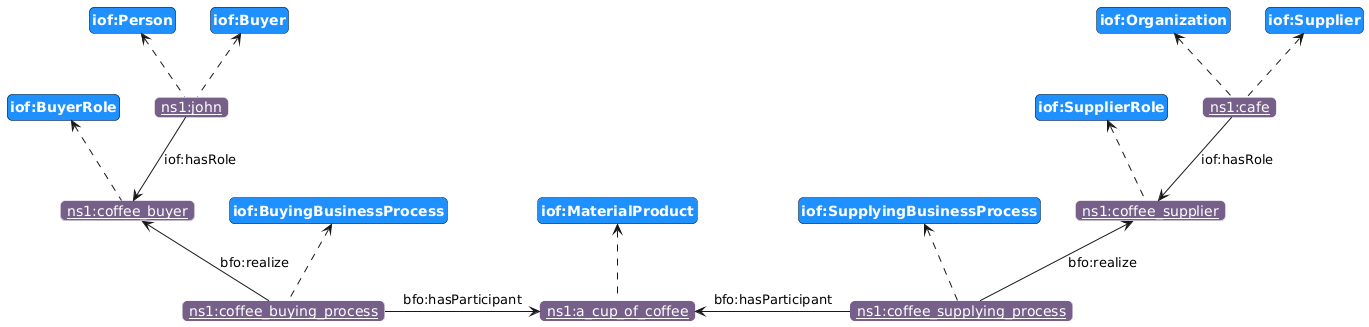
\includegraphics[scale=0.35]{scenarios/different-type-agent/image/different-type-agent.png}


\subsubsection*{Use-Case Example Data}


\begin{table}[h]
% \caption{}
\label{tab:organization-structure}
% \resizebox{\columnwidth}{!}{%
\begin{tabular}{|l|l|}
\hline

\hline
\end{tabular}%
% }
\end{table}


\subsubsection*{Data Mapping}
\begin{verbatim}

\end{verbatim}



\subsubsection*{Data Validation}


\chapter{System and organization}

\section{Different types of organisations}
\label{chapter-scenario-template}
\textbf{Created by:} Perawit Charoenwut \\
\textbf{Modified by:}

\subsection*{Scenario Objective}
This scenario illustrates how to represent a complete company structure with manufacturing and business divisions using the IOF core ontology. It focuses on:
\begin{itemize}
    \item Showing how business and manufacturing units coexist within one company
    \item Distinguishing between business and manufacturing activities
    \item Capturing different organizational roles and functions
\end{itemize}

\subsection*{General Pattern Description}
A company can contain both business organizations and manufacturers as part of its structure.
An Organization can simultaneously be:
\begin{enumerate}
    \item A BusinessOrganization that has a BusinessFunction, which is realized through a SellingBusinessProcess that sells the MaterialProduct
    \item A Manufacturer that has a ManufacturerRole, which is realized through a ProductProductionProcess and  has the MaterialProduct as its output.
\end{enumerate}

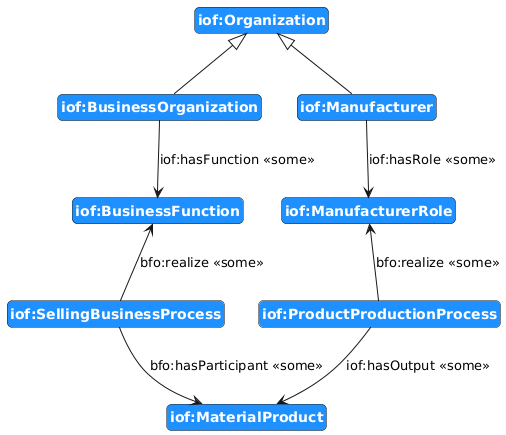
\includegraphics[scale=0.6]{scenarios/different-type-organizations/image/different-type-organizations-schema}

\subsection*{Use Case: }

This use case demonstrates how a company like GE operates as both a manufacturer and a business organization using the same material products.

\subsubsection*{Use-Case Pattern Description}
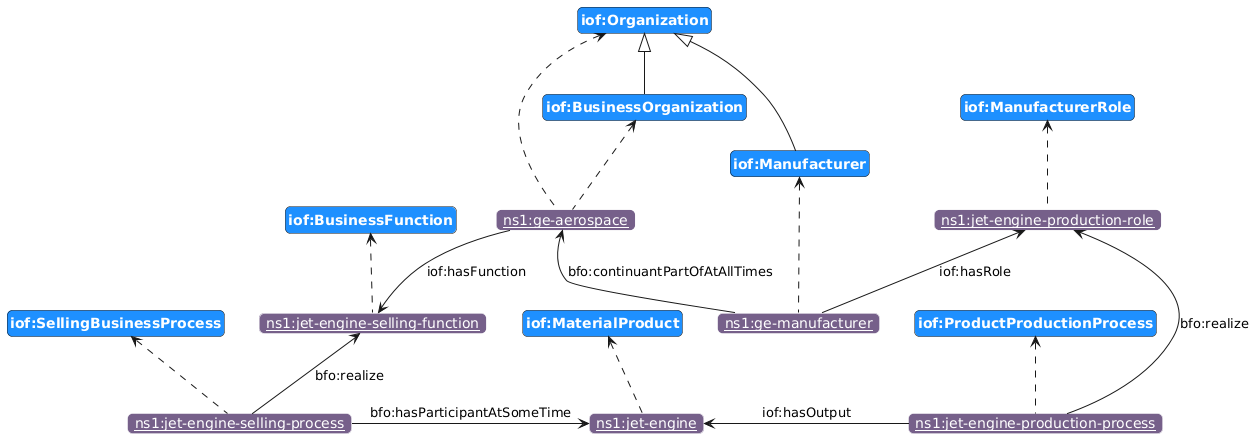
\includegraphics[scale=0.35]{scenarios/different-type-organizations/image/different-type-organizations}

GE Aerospace (\texttt{ns1:ge-aerospace}) operates as both an organization (\texttt{iof:Organization}) and a business organization (\texttt{iof:BusinessOrganization}) with respect to jet engines (\texttt{ns1:jet-engine}). Through its manufacturing division (\texttt{ns1:ge-manufacturer}), which is \texttt{bfo:continuantPartOfAtAllTimes} of GE Aerospace, it bears a manufacturer role (\texttt{ns1:jet-engine-production-role}) which is \texttt{bfo:realize} through a production process (\texttt{ns1:jet-engine-production-process}), producing jet engines as \texttt{iof:hasOutput}. The organization also has a business function (\texttt{ns1:jet-engine-selling-function}) which is \texttt{bfo:realize} through a selling process (\texttt{ns1:jet-engine-selling-process}), where the same jet engines are sold (\texttt{bfo:hasParticipantAtSomeTime}) in the selling process.
\subsubsection*{Use-Case Example Data}


\begin{table}[h]
% \caption{}
\label{tab:organization-structure}
% \resizebox{\columnwidth}{!}{%
\begin{tabular}{|l|l|}
\hline
Entity & Function/Role \\ \hline
GE Aerospace & Sells products and has Manufacturer \\
GE Manufacturer & Manufactures products \\
Jet engine & Product \\
\hline
\end{tabular}%
% }
\end{table}


\subsubsection*{Data Mapping}
\begin{verbatim}
INSERT DATA {
    ns1:ge-aerospace a iof:Organization, iof:BusinessOrganization;
        iof:hasFunction ns1:jet-engine-selling-function.
    
    ns1:ge-manufacturer a iof:Manufacturer;
        bfo:continuantPartOfAtAllTimes ns1:ge-aerospace;
        iof:hasRole ns1:jet-engine-production-role.
    
    ns1:jet-engine-selling-function a iof:BusinessFunction.
    ns1:jet-engine-selling-process a iof:SellingBusinessProcess;
        bfo:realize ns1:jet-engine-selling-function;
        bfo:hasParticipantAtSomeTime ns1:jet-engine.
    
    ns1:jet-engine-production-role a iof:ManufacturerRole.
    ns1:jet-engine-production-process a iof:ProductProductionProcess;
        bfo:realize ns1:jet-engine-production-role;
        iof:hasOutput ns1:jet-engine.
    
    ns1:jet-engine a iof:MaterialProduct.
    
    iof:BusinessOrganization rdfs:subClassOf iof:Organization.
    iof:Manufacturer rdfs:subClassOf iof:Organization.
}
\end{verbatim}



\subsubsection*{Data Validation}
\begin{verbatim}
#Shape for iof:BusinessOrganization
ns1:BusinessOrganizationShape a sh:NodeShape ;
    sh:targetClass iof:BusinessOrganization ;
    sh:property [
        sh:path iof:hasFunction ;
        sh:class iof:BusinessFunction ;
        sh:minCount 1 ;
    ] ;
    sh:property [
        sh:path rdfs:subClassOf ;
        sh:hasValue iof:Organization ;
    ] .

#Shape for Manufacturer
ns1:ManufacturerShape a sh:NodeShape ;
    sh:targetClass iof:Manufacturer ;
    sh:property [
        sh:path iof:hasRole ;
        sh:class iof:ManufacturerRole ;
        sh:minCount 1 ;
    ] ;
    sh:property [
        sh:path rdfs:subClassOf ;
        sh:hasValue iof:Organization ;
    ] .

# Shape for SellingBusinessProcess
ns1:SellingBusinessProcessShape a sh:NodeShape ;
    sh:targetClass iof:SellingBusinessProcess ;
    sh:property [
        sh:path bfo:realize ;
        sh:class iof:BusinessFunction ;
        sh:minCount 1 ;
    ] ;
    sh:property [
        sh:path bfo:hasParticipantAtSomeTime ;
        sh:class iof:MaterialProduct ;
        sh:minCount 1 ;
    ] .

# Shape for ProductProductionProcess
ns1:ProductProductionProcessShape a sh:NodeShape ;
    sh:targetClass iof:ProductProductionProcess ;
    sh:property [
        sh:path bfo:realize ;
        sh:class iof:ManufacturerRole ;
        sh:minCount 1 ;xf
    ] ;
    sh:property [
        sh:path iof:hasOutput ;
        sh:class iof:MaterialProduct ;
        sh:minCount 1 ;
    ] .
\end{verbatim}


\section{System and subsystem}





\chapter{Role}

\section{Gain and loss of roles}

\textbf{Created by:} Arkopaul Sarkar \\
\textbf{Modified by:} Arkopaul Sarkar \\

\subsection*{Scenario Objective}

BFO roles are realizable entities external to the bearer and assigned within specific physical, social, or institutional contexts. A bearer can hold multiple roles over time or simultaneously, without ceasing to exist when roles change. However, BFO lacks constructs to indicate when roles begin or end. This scenario discussed the patterns around two subclasses of bfo:process, introduced by IOF Core to represent the the start and end of role. 

\subsection*{General Pattern Description}



\includesvg[scale=0.6]{scenarios/role-gain-loss/images/general-pattern.svg}


\subsection*{Use Case: <Use-Case title>}
 \textit{ 
Describe a concrete use case for the pattern. (Multiple use cases can be described for one pattern. If multiple, please use distinct use case titles and repeat all subsubsections for each use case.)
  }

\subsubsection*{Use-Case Pattern Description}
 \textit{ 
Provide a diagram which matches the use-case pattern description. \\
\noindent \textit{This diagram is generally an object diagram. Please see examples of object diagram here.}
  }

 \textit{ 
Describe how the general pattern is applied to the use case. It is important to highlight within the description how the use-case-specific concepts align with the general pattern (e.g., SubClassOf Class for general pattern).
  }

\subsubsection*{Use-Case Example Data}
 \textit{ 
Provide a description of the data set used to demonstrate the use case pattern (e.g., format as JSON, CSV, XML, column/attribute/node name and their description, relation between datasets if multiple are used). Use not less than 3 and not more than 7 records/transactions.
  }

\subsubsection*{Data Mapping}
 \textit{ 
Describe how the data was mapped to RDF. Provide an INSERT DATA/ INSERT SPARQL for mapping. Use INSERT only when the use case example data needs further manipulation. \\
For INSERT DATA SPARQL, use only 2/3 records/transactions with named class and individuals. \\
For INSERT SPARQL, declare column names by `\{ \}' to the variable.  
For INSERT query, 
For both, do not use blank nodes.    
  }

\subsubsection*{Data Validation}
 \textit{ 
Data validation can be performed in two ways: accessing interesting facts using SPARQL or validating whether the entire data conforms to the ontology using SHACL. It is preferable to provide both. \\
Provide the SPARQL query in the code block along with the result of the query. \\
  }
\chapter{Changes}
\section{Change of object's location over time}
\label{sec-change-location}

\textbf{Created by:} Arkopaul Sarkar \\
\textbf{Modified by:} Arkopaul Sarkar \\

\subsection*{Scenario Objective}

This scenario illustrates how to represent the change in an object's physical location over time using the IOF/BFO ontology framework. It focuses on:
\begin{itemize}
    \item Emphasizing physical locations as sites and their association with spatial regions.
    \item Capturing actual movements of objects between existing locations (does not express any future plan or schedule of movement).
    \item \textbf{Temporal focus:} Associating specific temporal instants with the object's presence at particular locations.
\end{itemize}

\subsection*{General Pattern Description}
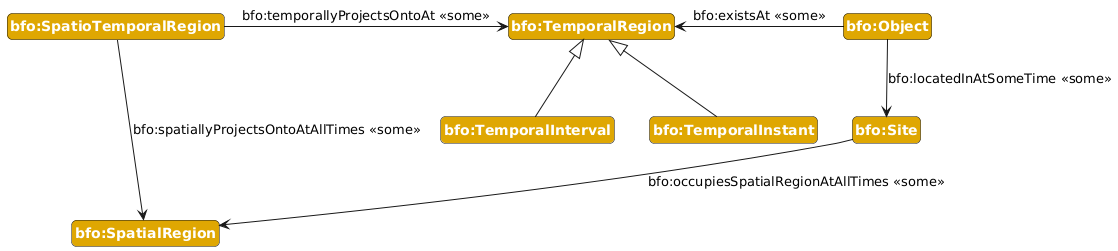
\includegraphics[scale=0.38]{scenarios/location-change/images/change-of-location-general.png}

An object may be located in different places at different times. In this scenario, the object can be related to multiple locations as \texttt{bfo:Site} by the \texttt{bfo:locatedInAtSomeTime} property. Similarly, the object can be related to multiple instances of \texttt{bfo:TemporalRegion}, each being either a \texttt{bfo:TemporalInterval} or a \texttt{bfo:TemporalInstant} by the \texttt{bfo:existsAt} property. As the object cannot be at two different locations at the same time, the times and the locations need to be paired up to denote at which location the object was at what time. Each pairing can be done by a different \texttt{bfo:SpatioTemporalRegion}. Following the 4D ontology of BFO, the object's spatial and temporal co-occupation can be represented by a \texttt{bfo:SpationTemporalRegion}, which \texttt{bfo:temporallyProjectsOnto} the temporal region the object exists at and \texttt{bfo:spatiallyProjectsOntoAtAllTimes} the \texttt{bfo:SpatialRegion} the object occupies (\texttt{occupiesSpatialRegionAtAllTimes}). 

Note that the pattern shows that it is the object's location (a \texttt{bfo:Site}) that \texttt{occupiesSpatialRegion\\AtAllTimes}. However, an object also occupies the same spatial region that its location occupies. Therefore, this pattern can also be used by directly relating the object to a spatial region by \texttt{occupiesSpa\\tialRegionAtAllTimes}. The choice depends on the kind of location, which is detailed in \cref{?chapter-space-location}.   

Note further that a \texttt{SpatioTemporalRegion} cannot project onto two or more different instances of \texttt{bfo:SpatialRegion} while projecting on a single \texttt{bfo:TemporalRegion}, as an object cannot be at two different locations at the same time. But it can be in the same location at different times. Therefore, a \texttt{SpatioTemporalRegion} can project onto two or more different instances of \texttt{bfo:TemporalRegion} while projecting onto a single \texttt{bfo:SpatialRegion}. However, the data mapping becomes easier if one pair of temporal and spatial regions is related to each spatio-temporal region. If the object is in the same location at different times, two spatio-temporal regions can relate each temporal region to the same spatial region. Observe that these two spatio-temporal regions are simply parts of the spatio-temporal region that projects onto two temporal regions. Therefore, they capture the same semantics while making data mapping easier.     

\subsubsection*{Use Case: Freight Train Location Change} 
A freight train operated by BNSF Railway hauls coal from Powder River Basin, Wyoming, to the Port of Long Beach in California. It was located at Powder River Basin station at 11:00 AM on Wednesday and then at Long Beach station at midnight on Thursday.

\subsubsection*{Use-Case Pattern Description}
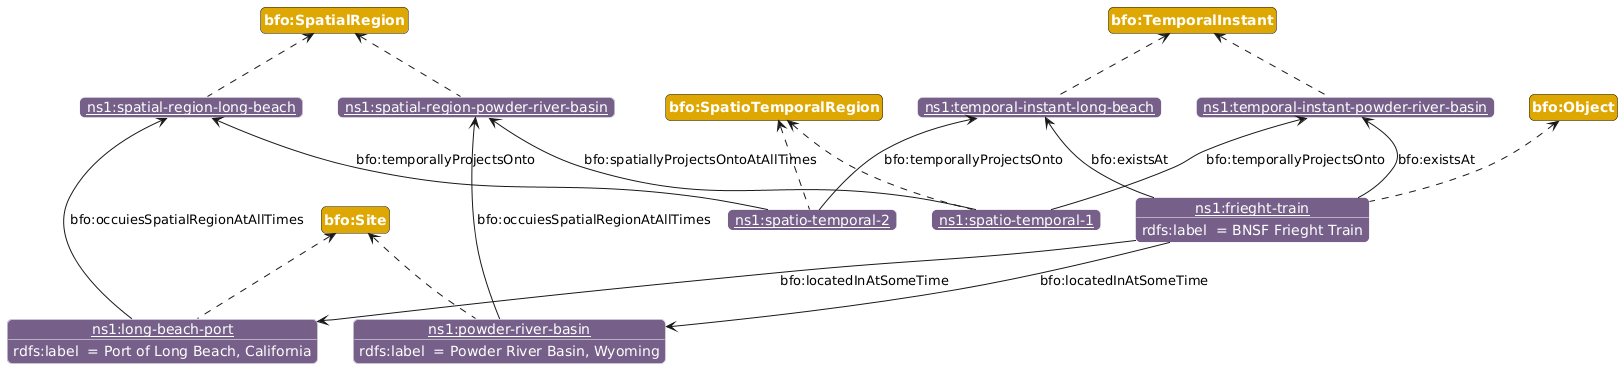
\includegraphics[scale=0.27]{scenarios/location-change/images/change-of-location-usecase1.png}
\begin{itemize}
    \item The train \texttt{ns1:freight-train} is located at (\texttt{bfo:locatedInAtSomeTime}) two different locations: \texttt{ns1:powder-river-basin} and \texttt{ns1:long-beach-port}, both of which are instances of \texttt{bfo:site}.
    \item Two separate instances of \texttt{bfo:SpatialRegion}: \texttt{ns1:spatial-region-powder-river-basin} and \texttt{ns1:spatial-region-long-beach}.
    \item The sites are linked to the spatial regions by \texttt{occupiesSpatialRegionAtAllTimes}.
    \item Temporal instants are linked to the sites, but the actual clock times are omitted for brevity.
\end{itemize}

\subsubsection*{Use-Case Example Data}

\begin{table}[h]
% \caption{}
\label{tab:freight-train-timetable}
\resizebox{\columnwidth}{!}{%
\begin{tabular}{|l|l|l|l|l|}
\hline
Train Number & Source             & Destination        & Departure Time & Arrival Time \\ \hline
31087        & Powder River Basin & Long Beach         & 11:00 AM       & 00:00 PM     \\
60123        & Long Beach         & Powder River Basin & 8:00 AM        & 1:00 PM      \\
31087        & Powder River Basin & Long Beach         & 10:00 AM       & 4:00 PM      \\
60123        & Long Beach         & Powder River Basin & 8:00 AM        & 1:00 PM      \\ \hline
\end{tabular}%
}
\end{table}

\subsubsection*{Data Mapping Description}

\begin{verbatim}
INSERT DATA {
    ns1:long-beach a bfo:Site; 
                      bfo:occupiesSpatialRegionAtAllTimes ns1:spatial-region-long-beach.
    ns1:powder-river-basin a bfo:Site; 
                      bfo:occupiesSpatialRegionAtAllTimes ns1:spatial-region-powder-river-basin.
    ns1:spatial-region-long-beach a bfo:SpatialRegion.
    ns1:spatial-region-powder-river-basin a bfo:SpatialRegion.
    ns1:temporal-instant-departure a bfo:TemporalInstant.
    ns1:temporal-instant-arrival a bfo:TemporalInstant.
    ns1:spatio-temporal-1 a bfo:SpatioTemporalRegion;
                      bfo:temporallyProjectsOnto ns1:temporal-instant-powder-river-basin;
                      bfo:temporallyProjectsOnto ns1:temporal-instant-long-beach;
                      bfo:spatiallyProjectsOntoAtAllTimes ns1:spatial-region-long-beach;
                      bfo:spatiallyProjectsOntoAtAllTimes ns1:spatial-region-powder-river-basin. 
    ns1:freight-train a bfo:Object;
                      rdfs:label "BNSF Freight Train";   
                      bfo:locatedInAtSomeTime ns1:powder-river-basin;
                      bfo:locatedInAtSomeTime ns1:long-beach-port;
                      bfo:existsAt ns1:temporal-instant-powder-river-basin;
                      bfo:existsAt ns1:temporal-instant-long-beach.               
}
\end{verbatim}
\noindent\rule{\linewidth}{0.1pt}
\begin{verbatim}
INSERT {
    _:source a bfo:Site; 
                      iof:hasValueExpressionAtAllTimes ?location1; 
                      bfo:occupiesSpatialRegionAtAllTimes _:spatial-region-source.
    _:destination a bfo:Site; 
                      iof:hasValueExpressionAtAllTimes ?location2; 
                      bfo:occupiesSpatialRegionAtAllTimes _:spatial-region-destination.
    _:spatial-region-source a bfo:SpatialRegion.
    _:spatial-region-destination a bfo:SpatialRegion.
    _:temporal-instant-departure a bfo:TemporalInstant;
                      iof:hasValueExpressionAtAllTimes ?departure.
    _:temporal-instant-arrival a bfo:TemporalInstant;
                      iof:hasValueExpressionAtAllTimes ?arrival.
    _:spatio-temporal-1 a bfo:SpatioTemporalRegion;
                      bfo:temporallyProjectsOnto _:temporal-instant-departure;
                      bfo:spatiallyProjectsOntoAtAllTimes _:spatial-region-source. 
    _:spatio-temporal-2 a bfo:SpatioTemporalRegion;
                      bfo:temporallyProjectsOnto _:temporal-instant-arrival;
                      bfo:spatiallyProjectsOntoAtAllTimes _:spatial-region-destination.
    ?freight-train a bfo:Object;
                      rdfs:label "BNSF Freight Train";   
                      bfo:locatedInAtSomeTime _:source;
                      bfo:locatedInAtSomeTime _:destination;
                      bfo:existsAt _:temporal-instant-departure;
                      bfo:existsAt _:temporal-instant-arrival.              
}
WHERE{
    BIND(COLUMN("Train Number") as ?freight-train).
    BIND(COLUMN("Source") as ?location1).
    BIND(COLUMN("Destination") as ?location2).
    BIND(COLUMN("Departure Time") as ?departure).
    BIND(COLUMN("Arrival Time") as ?arrival).
}
\end{verbatim}

\subsubsection*{Data Validation}

\begin{verbatim}
# Shape for bfo:SpatioTemporalRegion
ns1:SpatioTemporalRegionShape a sh:NodeShape ;
    sh:targetClass bfo:SpatioTemporalRegion ;
    sh:property [
        sh:path bfo:temporallyProjectsOnto ;
        sh:class ns1:TemporalInstant ;
        sh:minCount 1 ;
        sh:maxCount 1 ;
    ] ;
    sh:property [
        sh:path bfo:spatiallyProjectsOntoAtAllTimes ;
        sh:class bfo:SpatialRegion ;
        sh:minCount 1 ;
        sh:maxCount 1 ;
    ] .

# Shape for the object
ns1:ObjectShape a sh:NodeShape ;
    sh:targetClass bfo:Object ;
    sh:property [
        sh:path bfo:locatedInAtSomeTime ;
        sh:or ( 
            [ sh:class bfo:Site ] ;
            [ sh:class bfo:SpatialRegion ]
        ) ;
        sh:minCount 1 ;
    ] ;
    sh:property [
        sh:path bfo:existsAt ;
        sh:class ns1:TemporalInstant ;
        sh:minCount 1 ;
    ] .

# Shape for bfo:Site (if ns1:ObjectShape has bfo:Site as the target of path bfo:locatedInAtSomeTime)
ns1:SiteShape a sh:NodeShape ;
    sh:targetClass bfo:Site ;
    sh:property [
        sh:path bfo:occupiesSpatialRegionAtAllTimes ;
        sh:class bfo:SpatialRegion ;
        sh:minCount 1 ;
    ] .

Q. 1: How many 
\end{verbatim}
\chapter{Process and Event}
\chapter{Task Division Example}
%\label{chapter:title}

\emph{If a task division is required, a simple template can be found below for convenience. Feel free to use, adapt or completely remove.}

\begin{table}[htb]
    \setlength\extrarowheight{4pt}
    \centering
    \caption{Distribution of the workload}
    \label{tab:taskdivision}
    \begin{tabularx}{\textwidth}{lXX}
        \toprule
        & Task & Student Name(s) \\
        \midrule
        & Summary & \\
        Chapter 1 & Introduction &  \\
        Chapter 2 &  & \\
        Chapter 3 &  & \\
        Chapter * &  & \\
        Chapter * & Conclusion &  \\
        \midrule
        & Editors & \\
        & CAD and Figures & \\
        & Document Design and Layout & \\
        \bottomrule
    \end{tabularx}
\end{table}

\section*{Process Design}
Here discuss how to represent a SysML / UML activity diagram in an IOF Ontology.
\section*{Process Design and Conformance}
 Here discuss how to classify time stamped events automatically as making coffee.
\section{Algorithm execution}
\label{sec-algorithm-execution}

\textbf{Created by:} Milos Drobnjakovic \\
\textbf{Modified by:} Milos Drobnjakovic \\

\subsection*{Scenario Objective}

This scenario depicts how to express executions of algorithms by using BFO/IOF ontology.

Specifically, this pattern focuses on algorithm executions which produce Information Content Entities (ICEs) as outputs. As such, algorithms that return no ‘outputs’ are not included in this pattern.

This scenario is limited to algorithms that are part of a software system.


\subsection*{General Pattern Description}
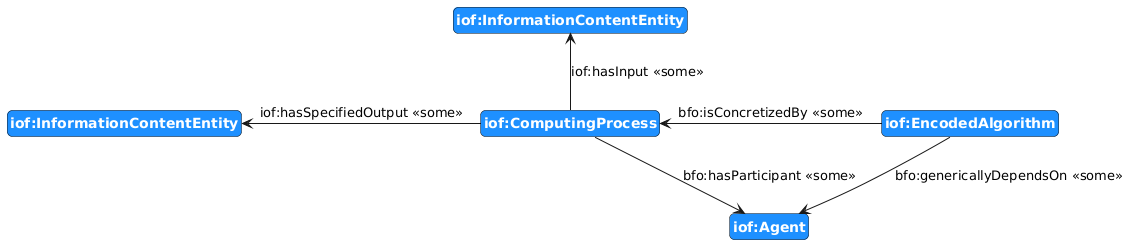
\includegraphics[scale=0.6]{scenarios/algorithm-execution/images/algorithm-execution-general.png}

...

\subsubsection*{Use Case: Drill failure prediction} 
A multilayer perceptron (MLP – a type of a neural network) is used to predict drill failure based on five measured parameters: ‘tool wear’, ‘air temperature’, ‘process temperature’, ‘torque’,’rotational speed’. The model uses the given parameters and outputs either ‘FAIL’ or ‘NOT FAIL’.

\subsubsection*{Use-Case Pattern Description}

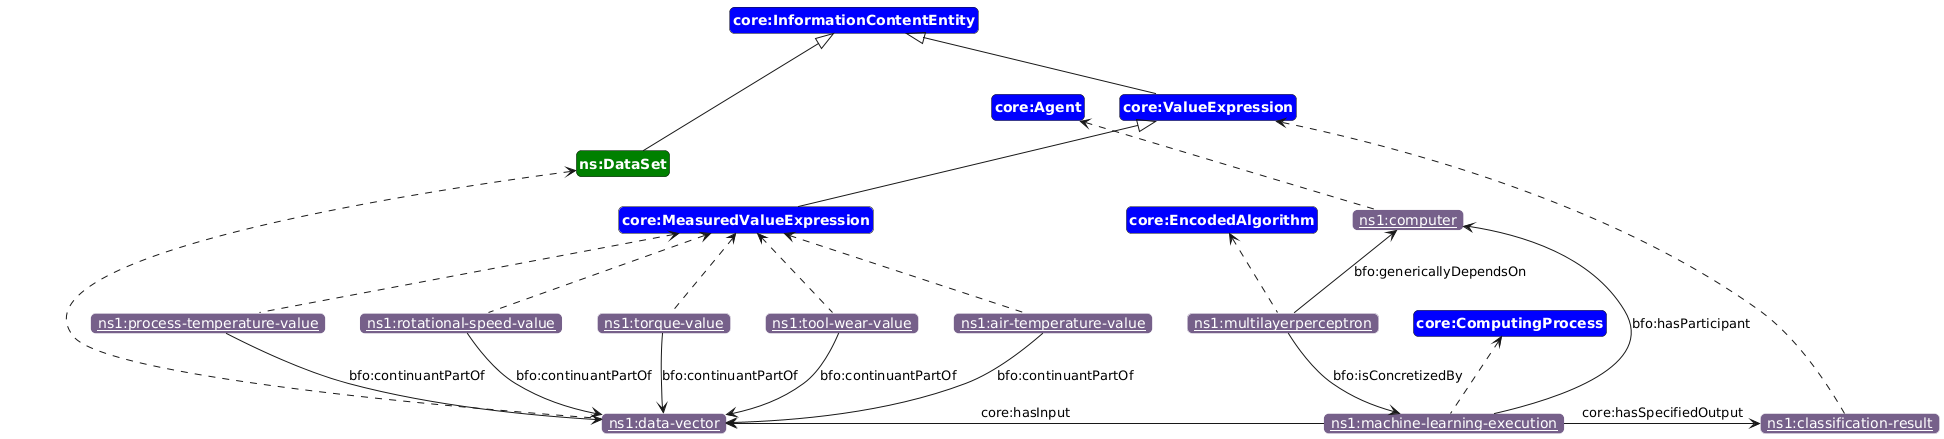
\includegraphics[scale=0.23]{scenarios/algorithm-execution/images/algorithm-execution-usecase1.png}

The machine learning model (MultiLayerPerceptron1) - an instance of:Encoded Algorithm is being concretized in a model execution process - an instance of:Computing Process. The MLP generically depends on a computer system (in this case an instance of Agent) which participates in the model execution process. Model execution utilizes the measured values associated with the drill and the drilling process and produces a ClassificationResult which is an instance of a ValueExpression. Since the objective is to predict machine failure the ClassificationResult is a prediction of the DrillFunction. The ClassificationResult can have two values associated with hasSimpleExpressionValue: 1) FAIL or 2) NOT FAIL. On the diagram bellow an example with the FAIL value is given. For brevity purposes the actual measurement values and their units are excluded from the diagram. Also, the association of the measured values with “drill attributes” or the “drilling process” are omitted. For a detailed guide on connecting the measured values with different entties - the user should see (placeholder link).

\subsubsection*{Use-Case Example Data}

For this use case a publicly available dataset was used: Predictive Maintenance⚙️ 

The dataset is a single CSV table consisting of the columns: ‘tool wear’, ‘air temperature’, ‘process temperature’, ‘torque’,’rotational speed’, ‘process ID, ‘type’ and ‘product ID’, ‘failure type’.

\begin{tabularx}{\textwidth}{|l|X|X|X|X|X|X|X|X|X|X|}
\hline
UDI & Product ID & Type & Air temperature {[}K{]} & Process temperature {[}K{]} & Rotational speed {[}rpm{]} & Torque {[}Nm{]} & Tool wear {[}min{]} & Target & Failure Type \\ \hline
1   & M14860     & M    & 298.1                   & 308.6                       & 1551                       & 42.8            & 0                   & 0      & No Failure   \\
2   & L47181     & L    & 298.2                   & 308.7                       & 1408                       & 46.3            & 3                   & 0      & No Failure   \\
3   & L47182     & L    & 298.1                   & 308.5                       & 1498                       & 49.4            & 5                   & 0      & No Failure   \\ \hline
\end{tabularx}

For prediction purposes, type and Product ID are omitted and are as such not included in the RDF. The exact type of failure is not utilized in this UC, since the model target is binary classification. Finally, `process id' is utilized for IRI construction of the drill.

\subsubsection*{Data Mapping Description}

\begin{verbatim}
INSERT DATA {
    <http://example.org/ns1:freight-train> a <http://example.org/bfo:Entity>;
    <http://example.org/ns1:freight-train> <http://example.org/bfo:locatedInAtSomeTime> 
        <http://example.org/ns1:powder-river-basin>.
}
\end{verbatim}

\subsubsection*{Data Validation}
\input{mainmatter/state-situation}
\chapter{Information}

\section{Information about some enttity(s)}
\label{sec-information-about}

\textbf{Created by:} Arkopaul Sarkar \\
\textbf{Modified by:}

\subsection*{Scenario Objective}
This scenario illustrates how various types of information about an entity (e.g., object, process, properties) can be captured. This scenario introduces the fundamental classes and properties to model information. Although IOF contains many types of informational entities, this scenario only introduces the generic types of information based on how they refer to the entities they are about.  

\subsection*{General Pattern Description}


\includegraphics[scale=0.5]{scenarios/object-artifact-material/image/what-is-made-of-schema.png}

The primitive and generic relationship \texttt{iof:isAbout} establishes a connection between an Information Content Entity (ICE) and a referenced entity, encapsulating the fundamental notion of ``aboutness''—that is, the ICE instance conveys information about the entity.

Three distinct modes of referring to an entity are captured through three specialized sub-properties of \texttt{iof:isAbout}: \texttt{iof:denotes} serves to distinguish one or more instances of an entity.
\texttt{iof:designates}, a functional specialization of \texttt{iof:denotes}, uniquely identifies a single specific instance, ensuring exclusive reference.
\texttt{iof:describes} conveys attributes or characteristics of an entity without necessarily providing unique identification. It emphasizes detailing the entity rather than establishing a direct referential link.
\texttt{iof:prescribes} refers to entities that may not yet exist but are expected to adhere to prescribed rules, guidelines, or specifications once instantiated. It thus encompasses potential future entities, such as artifacts constructed according to a design specification or processes executed in alignment with a plan specification.
Accordingly, the IOF Core ontology defines three corresponding classes of ICE—Designative ICE, Descriptive ICE, and Prescriptive ICE—each characterized based on these three sub-properties of \texttt{iof:isAbout}. 

\subsection*{Use Case Pattern Description}



\subsubsection*{Use-Case Example Data}


\subsubsection*{Data Mapping}


\subsubsection*{Data Validation}


URI of a website; social security number of a person (living in the United States), a global location number assigned to the Amazon regional distribution center at 12300 Bermuda Rd in Henderson, NV; the lot identifier assigned to a batch of rivets just received from China by the Airbus final assembly plant in Toulouse, FR; the VIN number assigned to the Tesla in my garage; a credit card number, the value of a field in a company's internal IT systems system used to uniquely identify a particular product and product revision.

Batch RV123456 - Rivets from China Lot number: RV123456
Supplier: China Aerospace Rivets Ltd. 

\section{descriptions}

We have to address:

simple description. e.g., name, ,,,

Value expressions. subtypes of value expressions

1cm is the value expression of the diameter of a screw head that is specified in its design; 37C is the value expression of the temperature of a bioreactor measured during the production process; "low risk" is the value expression of a process parameter based on the risk analysis classification scheme; 3 g/l is the value expression of titer of an antibody generated by a process simulation - need to be genric...


\section{Plan Specification}



\section{Design specification}



\section{Service Agreement}
\input{mainmatter/planning}
\chapter{Measurement}

\section{Simple vs Aggregate Measurement}

\section{Unitless measurements}
count, percentage. ratio

\section{Multiple measurements of the same object at the same time}
different measurement processes 
measurements using different instruments

\section{Time-series measurement}
(process characteristics)

\section{uncertainty, range of values}
if time permits


\input{mainmatter/utility}

%% Prevent urls running into margins in bibliography
\setcounter{biburlnumpenalty}{7000}
\setcounter{biburllcpenalty}{7000}
\setcounter{biburlucpenalty}{7000}

%% Add bibliography
\printbibliography[heading=bibintoc,title=References]

%% ----------------------------------------------------------------------
%%    Appendix (Letters for chapters)
%% ----------------------------------------------------------------------

\appendix

\chapter{Instructions to the authors}


\chapter{Scenerio Template}
\textit{This template should be used to create a scenario. Please copy to a dedicated folder under folder `scenario'. All images should be referred from `image' folder under the dedicated folder. For example, please see: \\
\cref{sec-change-location}}

\section*{<Scenario title>}
\addcontentsline{toc}{section}{Basic Formal Ontology}

\textit{Short Phrase (e.g., Change of object's location over time)}

\textbf{Created by:} Arkopaul Sarkar \\
\textbf{Modified by:} Arkopaul Sarkar \\

\subsection*{Scenario Objective}
% Instruction box
\textit{ 
Describe the general purpose of representing the pattern (e.g., demonstrating how you can depict measurements with IOF core).}


\subsection*{General Pattern Figure}
\textit{  
Provide a figure containing the pattern independent of the use case (e.g., just measurements in general as opposed to measuring a particular thing such as pH or length). \\
\noindent \textit{This diagram is generally a simple class-relation diagram. Please see examples of class-relation diagram here.}
  }


\subsection*{General Pattern Description}
\textit{ 
Describe the general pattern, including any background why such types and relations are used. Also mention any alternative or shortcuts. Please provide a background of the types and relations in the context of IOF (please prefer logical arguments to didactic arguments).
}


\subsection*{Use Case: <Use-Case title>}
 \textit{ 
Describe a concrete use case for the pattern. (Multiple use cases can be described for one pattern. If multiple, please use distinct use case titles and repeat all subsubsections for each use case.)
  }

\subsubsection*{Use-Case Diagram}
 \textit{ 
Provide a diagram which matches the use-case pattern description. \\
\noindent \textit{This diagram is generally an object diagram. Please see examples of object diagram here.}
  }

\subsubsection*{Use-Case Pattern Description}
 \textit{ 
Describe how the general pattern is applied to the use case. It is important to highlight within the description how the use-case-specific concepts align with the general pattern (e.g., SubClassOf Class for general pattern).
  }

\subsubsection*{Use-Case Example Data}
 \textit{ 
Provide a description of the data set used to demonstrate the use case pattern (e.g., format as JSON, CSV, XML, column/attribute/node name and their description, relation between datasets if multiple are used). Use not less than 3 and not more than 7 records/transactions.
  }

\subsubsection*{Data Mapping}
 \textit{ 
Describe how the data was mapped to RDF. Provide an INSERT DATA/ INSERT SPARQL for mapping. Use INSERT only when the use case example data needs further manipulation. \\
For INSERT DATA SPARQL, use only 2/3 records/transactions with named class and individuals. \\
For INSERT SPARQL, declare column names by `\{ \}' to the variable.  
For INSERT query, 
For both, do not use blank nodes.    
  }

\subsubsection*{Data Validation}
 \textit{ 
Data validation can be performed in two ways: accessing interesting facts using SPARQL or validating whether the entire data conforms to the ontology using SHACL. It is preferable to provide both. \\
Provide the SPARQL query in the code block along with the result of the query. \\
  }
\chapter{About the Template}
%\label{chapter:title}

This template aims to simplify and improve the (Xe)LaTeX report/thesis template by Delft University of Technology with the following three main design principles:

\begin{itemize}
  \item \textbf{Simplicity First:} A class file that has been reduced by nearly 70\% to simplify customization;
  \item \textbf{Effortless:} A careful selection of common packages to get started immediately;
  \item \textbf{Complete:} Ready-to-go when it comes to the document and file structure.
\end{itemize}

\noindent This template works with pdfLaTeX, XeLaTeX and LuaLaTeX. In order to adhere to the TU Delft house style, either XeLaTeX or LuaLaTeX is required, as it supports TrueType and OpenType fonts. BibLaTeX is used for the bibliography with as backend biber. Please visit \url{https://dzwaneveld.github.io/report/} for the full documentation.

\section*{Documentation (Abridged)}

As a report/thesis is generally a substantial document, the chapters and appendices have been separated into different files and folders for convenience. The folders are based on the three parts in the document: the frontmatter, mainmatter and appendix. All files are inserted in the main file, \texttt{report.tex}, using the \texttt{\textbackslash input\{filename\}} command. The document class, which can be found in \texttt{tudelft-report.cls}, is based on the book class. 

The template will automatically generate a cover when the \texttt{\textbackslash makecover} command is used. The title, subtitle and author will also be present on the title page. To give greater flexibility over the title page, the layout is specified in \texttt{title-report.tex}. A title page for theses is also available: \texttt{title-thesis.tex}. Change the corresponding \texttt{\textbackslash input\{...\}} command in the main file to switch. 

The bibliography has been set up in \texttt{report.tex} to allow for easy customization. It is included in the table of contents and renamed to 'References' using the \texttt{heading=bibintoc} and \texttt{title=References} options of the \texttt{\textbackslash printbibliography} command respectively. If you would like to use a different .bib file, change the command \texttt{\textbackslash addbibresource{report.bib}} accordingly.

\emph{→ Visit \url{https://dzwaneveld.github.io/report/} for the full documentation.}

\section*{License}

This template by Daan Zwaneveld is licensed under CC BY-NC 4.0. To view a copy of this license, visit \url{https://creativecommons.org/licenses/by-nc/4.0/}. No attribution is required in PDF outputs created using this template.
\end{document}
